% !TeX document-id = {162e9e21-9983-435d-9452-f8de7c260717}
% !TeX program = lualatex
% !BIB TS-program = biber
\documentclass[10pt,aspectratio=169,english]{beamer}
\usepackage{graphicx} % Required for inserting images
\usepackage{caption}
\usepackage{subcaption}
\usepackage{complexity}
\usepackage{framed}

%\usepackage[charter]{mathdesign}
% \usepackage{xcharter-otf}
% \usepackage{hologo}
% \usepackage{luamesh}

\usepackage[english]{babel}
\usepackage{tcolorbox}
\usepackage[style=authoryear, backend=biber]{biblatex}
\usepackage{cleveref}
% \hypersetup{colorlinks=true}

\usepackage{tikz}
\usetikzlibrary {graphs, graphs.standard, graphdrawing}
\usegdlibrary {circular}
\usegdlibrary{force}
\usegdlibrary{trees}

\pgfdeclareimage[width=6mm]{tree}{tree}
\pgfdeclareimage[width=5mm]{fire}{fire}
\pgfdeclareimage[width=6mm]{fighter}{fighter}

%\usepackage{beamerthemeAmurmaple}

\tcbuselibrary{listings,breakable}
\tcbuselibrary{documentation}
\tcbset{
  color command=AmurmapleRed,
  color environment=AmurmapleRed,
  color option=AmurmapleGreen
}

%\usepackage{cmbright}

\usetheme[
%nogauge,
nomail,
%delaunay,
%amurmapleblue
]{Amurmaple}

\lstset{
  numberstyle=\footnotesize\color{gray},
  keywordstyle=\ttfamily\bfseries\color{structure},
  basicstyle=\ttfamily\normalsize,
  commentstyle=\itshape\color{gray},
  stringstyle=\ttfamily,
  showstringspaces=false,
  language=[LaTeX]TeX,
  breaklines=true,
  breakindent=30pt,
  defaultdialect=[LaTeX]TeX,
  morekeywords={usetheme,definecolor, beamerbutton, beamerskipbutton,
    beamerreturnbutton, structure, alert, sectionpage, mail, webpage,
    collaboration, subtitle, institute, titlegraphic, sepframe, includegraphics,
    thanksframe, inserttitlegraphic, framesection, boxalert,appendix,logo}
  % frame=tb
}

\newtcblisting{Code}{%
  arc=0pt,outer arc=0pt,
  colback=structure!3,
  colframe=structure,
  breakable,
  boxsep=0pt,left=5pt,right=5pt,top=5pt,bottom=5pt, bottomtitle =
  3pt, toptitle=3pt,
  boxrule=0pt,bottomrule=0.5pt,toprule=0.5pt, toprule at break =
  0pt, bottomrule at break = 0pt,
  listing options={breaklines,basicstyle=\ttfamily},listing only,
}

\newtcblisting{Exemple}{%
  arc=0pt,outer arc=0pt,
  colback=structure!3,
  colframe=structure,
  breakable,
  boxsep=0pt,left=3pt,right=3pt,top=2pt,bottom=2pt, bottomtitle =
  0pt, toptitle=0pt,
  boxrule=0pt,bottomrule=0.5pt,toprule=0.5pt, toprule at break =
  0pt, bottomrule at break = 0pt,
  listing options={breaklines,basicstyle=\ttfamily},
}

\newtcblisting{CodePreambule}{%
  arc=0pt,outer arc=0pt,
  colback=AmurmapleBlue!5,
  colframe=AmurmapleBlue,
  breakable,
  boxsep=0pt,left=5pt,right=5pt,top=5pt,bottom=5pt, bottomtitle =
  3pt, toptitle=3pt,
  boxrule=0pt,bottomrule=0.5pt,toprule=0.5pt, toprule at break =
  0pt, bottomrule at break = 0pt,
  enhanced,
  overlay  ={%
    \node[ minimum width=1cm,
      anchor=south east,yshift=-0cm,fill=AmurmapleBlue] at (frame.south east)
      {\itshape\color{white} preamble};
      % \node[ minimum width=1cm,
      % anchor=south east,yshift=-0cm,color=gray,opacity=0.7] at (frame.south east)
      % {\itshape\small préambule};
  },
  listing options={
    breaklines,
    basicstyle=\ttfamily,
  },listing only,
}


\title[Restricting infections on graph classes]{Restricting infections on graph classes}
\author[S.~Santos]{Samuel Santos}
%\subtitle{Qualificação de Mestrado}
\institute[UFC]{UFC\\
Universidade Federal do Ceará}
\date{December 2024}
\titlegraphic{
\includegraphics[width=2.4cm]{ufc-logo.png}}
\mail{csamuelssm@alu.ufc.br}
%\webpage{www.ceremade.dauphine.fr/~chupin/}
\collaboration{Supervised by Ana Karolinna Maia de Oliveira and Carlos Vinícius Gomes Costa Lima}

\bibliography{biblio.bib}
\usefonttheme{default}
\DeclareMathVersion{sans}
\SetSymbolFont{operators}{sans}{OT1}{cmbr}{m}{n}
\SetSymbolFont{letters}{sans}{OML}{cmbrm}{m}{it}
\SetSymbolFont{symbols}{sans}{OMS}{cmbrs}{m}{n}
\SetMathAlphabet{\mathit}{sans}{OT1}{cmbr}{m}{sl}
\SetMathAlphabet{\mathbf}{sans}{OT1}{cmbr}{bx}{n}
\SetMathAlphabet{\mathtt}{sans}{OT1}{cmtl}{m}{n}
\SetSymbolFont{largesymbols}{sans}{OMX}{iwona}{m}{n}
\sffamily\mathversion{sans}
%\renewcommand{\familydefault}{\sfdefault}
%\renewcommand{\sfdefault}{cmbr}
%\renewcommand{\ttdefault}{cmbr}
%\usefonttheme{professionalfonts}

\begin{document}

\maketitle

\section{Introduction}

\begin{frame}{Introduction}

\onslide<1->{
    Several phenomena happen in a \textbf{contagion-like manner}.

    \begin{itemize}
        \item<1-> Spreading of pathogens, like viruses or bacteria;
        \item<2-> The diffusion of innovation, (mis-)information, and memes.
        \only<2>{
            \begin{information}
                Studies found that most people adopt innovative ideas based on the experience of their neighbors or community.
                \begin{itemize}
                    \item The adoption of hybrid seed corn among farmers \parencite{ryan2017acceptance};
                    \item The adoption of tetracycline by physicians \parencite{Coleman1957-tv}.
                \end{itemize}
            \end{information}
        }
        \item<3-> Even bedbugs seem to spread from hotel to hotel via travelers \parencite{barabasi2016network}.
    \end{itemize}
}

\end{frame}

\begin{frame}{Introduction}
    \onslide<1->{
        The early models built to study such phenomena are the so-called \textit{compartmental models}.
        \begin{itemize}
            \item Compartments are states;
            \item Each agent/individual belongs to one state.
        \end{itemize}
    }
    
    \only<2>{
        \begin{exampleblock}{Example (SIR)}
            \begin{figure}
                \centering
                \begin{subfigure}[c]{0.6\textwidth}
                    \centering
                    
\includegraphics[width=\textwidth]{SIR.png}
                \end{subfigure}\quad
                \begin{subfigure}[c]{0.25\textwidth}
                    \centering
                    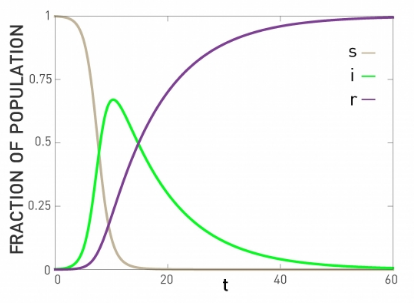
\includegraphics[width=\textwidth]{sir-graphic.png}
                \end{subfigure}
            \end{figure}
        \end{exampleblock}
    }

    \onslide<3->{
        \begin{definition}[Homogeneous Mixing Hypothesis]
            The assumption that every individual from one compartment has the same chance of interacting with an individual from another compartment.
        \end{definition}
    }

    \begin{itemize}
        \item<4-> The homogeneous mixing hypothesis is \textcolor{red}{\textbf{false}}.
        \item<5-> The \textbf{structure of the contact network} is what facilitates the contagion.
    \end{itemize}
    
    \only<5>{
    \begin{information}
    	Studies have shown that the airport mobility network provides reliable information for the prediction and control of airborne epidemics like H1N1 \parencite{SorianoPaos2022}.
    	\end{information}
    }
\end{frame}

\section{The Threshold Model}

\begin{frame}{Modeling Contagion on Graphs: Threshold Model}

\begin{itemize}
    \item<1-> Let's consider each vertex as an individual.
    \begin{itemize}
        \item<1-> A vertex is either \textbf{active (infected)} or \textbf{inactive (susceptible)}.
    \end{itemize}
    \item<2-> The individuals change their state based on their neighbors' state.
    \begin{itemize}
        \item<2-> A threshold value represents \textbf{how susceptible} an individual is to the contagious agent.
        \item<2-> Smaller thresholds: early adopters / low immunity;
        \item<4-> Bigger thresholds: laggards / greater resistance.
    \end{itemize}
\end{itemize}

\only<2>{
	\begin{figure}
		\centering
		\tikz \graph [spring layout, nodes={draw,circle}] { a[label=above:{\textcolor{red}{1}}] -- {u[fill=red], w, x[fill=red], y, z[fill=red]} };
	\end{figure}
}

\only<3>{
	\begin{figure}
		\centering
		\tikz \graph [spring layout, nodes={draw,circle}] { a[fill=red, label=above:{\textcolor{red}{1}}] -- {u[fill=red], w, x[fill=red], y, z[fill=red]} };
	\end{figure}
}

\only<4>{
	\begin{figure}
		\centering
		\tikz \graph [spring layout, nodes={draw,circle}] { a[label=above:{\textcolor{blue}{5}}] -- {u[fill=red], w, x[fill=red], y, z[fill=red]} };
	\end{figure}
}
    
\end{frame}

\begin{frame}{Modeling Contagion on Graphs: Threshold Model}
	In the threshold model, we are given:
	\begin{itemize}
		\item<1-> A \textbf{graph} $G=(V, E)$;
		\item<2-> A \textbf{threshold function} $t:V(G) \rightarrow \mathbb{N}$;
		\item<3-> A set of \textbf{initial infected vertices} -- the \textit{seed set} $S \subseteq V(G)$.
		\item<4-> The diffusion happens in \textbf{discrete time steps}.
		\item<6-> Once a vertex is infected, it \textbf{stays infected} -- we call it a \textbf{$t$-irreversible process}.
	\end{itemize}
	
	\only<1>{
		\begin{figure}
			\centering
			\tikz \graph [spring layout, nodes={draw,circle}, horizontal=a to g] {
				a -- {b, c};
				b -- {c, d, e};
				d -- {[clique] e, f, g}
			};
		\end{figure}
	}
	
	\only<2>{
		\begin{figure}
			\centering
			\tikz \graph [spring layout, nodes={draw,circle}, horizontal=a to g] {
				a[label=below:{\textcolor{red}{2}}] -- {b[label=left:{\textcolor{red}{3}}], c[label=above:{\textcolor{red}{1}}]};
				b -- {c, d, e[label=above:{\textcolor{red}{3}}]};
				d[label=below:{\textcolor{red}{1}}] -- {[clique] e, f[label=above:{\textcolor{red}{2}}], g[label=below:{\textcolor{red}{2}}]}
			};
		\end{figure}
	}
	
	\only<3-4>{
		\begin{figure}
			\centering
			\tikz \graph [spring layout, nodes={draw,circle}, horizontal=a to g] {
				a[fill=red, label=below:{\textcolor{red}{2}}] -- {b[label=left:{\textcolor{red}{3}}], c[label=above:{\textcolor{red}{1}}]};
				b -- {c, d, e[fill=red, label=above:{\textcolor{red}{3}}]};
				d[label=below:{\textcolor{red}{1}}] -- {[clique] e, f[label=above:{\textcolor{red}{2}}], g[label=below:{\textcolor{red}{2}}]};
			};
		\end{figure}
	}
	
	\only<5>{
		\begin{figure}
			\centering
			\tikz \graph [spring layout, nodes={draw,circle}, horizontal=a to g] {
				a[fill=red, label=below:{\textcolor{red}{2}}] -- {b[label=left:{\textcolor{red}{3}}], c[fill=red, label=above:{\textcolor{red}{1}}]};
				b -- {c, d[fill=red, label=below:{\textcolor{red}{1}}], e[fill=red, label=above:{\textcolor{red}{3}}]};
				d -- {[clique] e, f[label=above:{\textcolor{red}{2}}], g[label=below:{\textcolor{red}{2}}]};
			};
		\end{figure}
	}
	
	\only<6>{
		\begin{figure}
			\centering
			\tikz \graph [spring layout, nodes={draw,circle}, horizontal=a to g] {
				a[fill=red, label=below:{\textcolor{red}{2}}] -- {b[fill=red, label=left:{\textcolor{red}{3}}], c[fill=red, label=above:{\textcolor{red}{1}}]};
				
				b -- {c, d[fill=red, label=below:{\textcolor{red}{1}}], e[fill=red, label=above:{\textcolor{red}{3}}]};
				d -- {[clique] e, f[fill=red, label=above:{\textcolor{red}{2}}], g[fill=red, label=below:{\textcolor{red}{2}}]};
			};
		\end{figure}
	}
\end{frame}

\begin{frame}{Problems arising from the Threshold Model}
	Several computational problems arise from the Threshold Model.
	\begin{itemize}
		\item<1-> \textbf{Influence Maximization} (\textsc{IM}) \parencite{kempe}: find a seed set of bounded cardinality that maximizes the number of infected vertices.
		\begin{itemize}
			\item<2-> Decision version is \NP-complete even for bipartite graphs.
			\item<3-> \NP-complete even for $k$-regular graphs if we require $S$ to infect all vertices of $G$ -- \textbf{Target Set Selection} (\textsc{TSS}) \parencite{DREYER2009}.
		\end{itemize}
	\end{itemize}
\end{frame}

\begin{frame}{Problems arising from the Threshold Model}
	
	\onslide<1->{
		Variations of these problems:
		\begin{itemize}
			\item Directed version;
			\item Majority version: $t(v) = \lceil \frac{d(v)}{2} \rceil \quad \forall v \in V(G)$;
			\item \textsc{TSS} with maximum activation time \parencite{Keiler2023, Flocchini2003, Marcilon2018};
			\item \textsc{TSS} with activation time equal to~1 \parencite{Arajo2023};
		\end{itemize}
	}
\end{frame}

\begin{frame}{Problems arising from the Threshold Model}
	
	\textbf{Immunization problems}:
	
	\begin{itemize}
		\item<1-> \textbf{Firefighter};
		\begin{itemize}
			\item<2-> A fire breaks at some vertex and will spread;
			\item<3-> The goal is to place firefighters to protect the vertices from the fire.
			\item<6-> \NP-complete \textbf{even for trees!} (And a bunch of other classes)
		\end{itemize}
		\item<7-> \textbf{Influence Immunization Bounding} (\textsc{IIB});
		\begin{itemize}
			\item<7-> A generalization of Firefighter? \textbf{No, but sort of...}
		\end{itemize}
	\end{itemize}
	
	\only<2>{
		\begin{figure}
		\centering
		\begin{tikzpicture}
			\scoped [tree layout]
			\node {\pgfuseimage{fire}}
			child { node {\pgfuseimage{tree}} child { node {\pgfuseimage{tree}}} child { node {\pgfuseimage{tree}}  child { node {\pgfuseimage{tree}}} child { node {\pgfuseimage{tree}}}}  }
			child { node {\pgfuseimage{tree}}  child { node {\pgfuseimage{tree}}} child { node {\pgfuseimage{tree}}} child { node {\pgfuseimage{tree}}} };
		\end{tikzpicture}
		\end{figure}
	}
	
	\only<3>{
		\begin{figure}
			\centering
			\begin{tikzpicture}
				\scoped [tree layout]
				\node {\pgfuseimage{fire}}
				child { node {\pgfuseimage{tree}} child { node {\pgfuseimage{tree}}} child { node {\pgfuseimage{tree}}  child { node {\pgfuseimage{tree}}} child { node {\pgfuseimage{tree}}}}  }
				child { node {\pgfuseimage{fighter}}  child { node {\pgfuseimage{tree}}} child { node {\pgfuseimage{tree}}} child { node {\pgfuseimage{tree}}} };
			\end{tikzpicture}
		\end{figure}
	}
	
	\only<4>{
		\begin{figure}
			\centering
			\begin{tikzpicture}
				\scoped [tree layout]
				\node {\pgfuseimage{fire}}
				child { node {\pgfuseimage{fire}} child { node {\pgfuseimage{tree}}} child { node {\pgfuseimage{tree}}  child { node {\pgfuseimage{tree}}} child { node {\pgfuseimage{tree}}}}  }
				child { node {\pgfuseimage{fighter}}  child { node {\pgfuseimage{tree}}} child { node {\pgfuseimage{tree}}} child { node {\pgfuseimage{tree}}} };
			\end{tikzpicture}
		\end{figure}
	}
	
	\only<5>{
		\begin{figure}
			\centering
			\begin{tikzpicture}
				\scoped [tree layout]
				\node {\pgfuseimage{fire}}
				child { node {\pgfuseimage{fire}} child { node {\pgfuseimage{tree}}} child { node {\pgfuseimage{fighter}}  child { node {\pgfuseimage{tree}}} child { node {\pgfuseimage{tree}}}}  }
				child { node {\pgfuseimage{fighter}}  child { node {\pgfuseimage{tree}}} child { node {\pgfuseimage{tree}}} child { node {\pgfuseimage{tree}}} };
			\end{tikzpicture}
		\end{figure}
	}
	
	\only<6>{
		\begin{figure}
			\centering
			\begin{tikzpicture}
				\scoped [tree layout]
				\node {\pgfuseimage{fire}}
				child { node {\pgfuseimage{fire}} child { node {\pgfuseimage{fire}}} child { node {\pgfuseimage{fighter}}  child { node {\pgfuseimage{tree}}} child { node {\pgfuseimage{tree}}}}  }
				child { node {\pgfuseimage{fighter}}  child { node {\pgfuseimage{tree}}} child { node {\pgfuseimage{tree}}} child { node {\pgfuseimage{tree}}} };
			\end{tikzpicture}
		\end{figure}
	}
	
\end{frame}

\section{Influence Immunization Bounding}

\begin{frame}{Influence Immunization Bounding}
	First, we need to define what it means to \textbf{immunize a vertex}.
	
	\begin{itemize}
		\item<1-> Option 1: raise the vertex threshold above its degree;
		\item<4-> \only<4>{Option 2: make the vertex invisible -- remove it.}\only<5>{\textcolor{red}{\textbf{Option 2: make the vertex invisible -- remove it.}}}
	\end{itemize}
	
	\only<1>{
		\begin{figure}
			\centering
			\tikz \graph [spring layout, nodes={draw,circle}] { a[label=above:{\textcolor{red}{$+\infty$}}, draw=blue, line width=1mm] -- {u[fill=red], w[label=left:{\textcolor{red}{1}}], x[fill=red], y[label=right:{\textcolor{red}{1}}], z[fill=red]} };
		\end{figure}
	}
	
	\only<2>{
		\begin{minipage}[c]{0.5\textwidth}
			\begin{figure}
				\centering
				\tikz \graph [spring layout, nodes={draw,circle}] { a[label=above:{\textcolor{red}{3}}] -- {u[fill=red], w[label=left:{\textcolor{red}{1}}], x[label=left:{\textcolor{red}{$+\infty$}}, draw=blue, line width=1mm, fill=red], y[label=right:{\textcolor{red}{1}}], z[fill=red]} };
			\end{figure}
		\end{minipage}\begin{minipage}[c]{0.5\textwidth}
			\begin{remark}[Option 1]
				Infected vertices can also be immunized. In this option, the immunized infected vertices still \textbf{can infect others}.
			\end{remark}
		\end{minipage}
	}
	
	\only<3>{
		\begin{minipage}[c]{0.5\textwidth}
			\begin{figure}
				\centering
				\tikz \graph [spring layout, nodes={draw,circle}] { a[label=above:{\textcolor{red}{3}}, fill=red] -- {u[fill=red], w[label=left:{\textcolor{red}{1}}], x[label=left:{\textcolor{red}{$+\infty$}}, draw=blue, line width=1mm, fill=red], y[label=right:{\textcolor{red}{1}}], z[fill=red]} };
			\end{figure}
		\end{minipage}\begin{minipage}[c]{0.5\textwidth}
			\begin{remark}[Option 1]
				Infected vertices can also be immunized. In this option, the immunized infected vertices still \textbf{can infect others}.
			\end{remark}
		\end{minipage}
	}
	
	\only<4-5>{
		\begin{minipage}[c]{0.5\textwidth}
			\begin{figure}
				\centering
				\tikz \graph [spring layout, nodes={draw,circle}] {
					a --[dashed] x[label=left:{\textcolor{red}{$+\infty$}}, line width=1mm, fill=red, dashed, draw=blue];
					
					a[label=above:{\textcolor{red}{3}}] -- {u[fill=red], w[label=left:{\textcolor{red}{1}}], y[label=right:{\textcolor{red}{1}}], z[fill=red]};							
				};
				
			\end{figure}
		\end{minipage}\begin{minipage}[c]{0.5\textwidth}
			\begin{remark}[Option 2]
				In this option, immunized vertices do not infect nor get infected.
			\end{remark}
		\end{minipage}
	}
\end{frame}

\begin{frame}{Influence Immunization Bounding}
	
	\begin{minipage}[t]{0.6\textwidth}
		\onslide<1->{
			Given:
			\begin{itemize}
				\item<1-> A graph $G=(V, E)$ with thresholds $t:V(G) \rightarrow \mathbb{N}$;
				\item<2-> A seed set $S \subseteq V(G)$;
				\item<5-> Naturals $k$ and $l$. \only<6->{\textbf{Let $k=3$ and $l=2$.}}
			\end{itemize}
		}
		
		\onslide<6->{
			We want to find a immunizing set $Y \subseteq V(G)$ such that:
			\begin{itemize}
				\item<6-> $|Y| \leq l$; and
				\item<7-> By immunizing $Y$ at time $\tau=0$, the \textbf{infection gets restricted to at most $k$ vertices}.
			\end{itemize}
		}
		
		\only<2-4>{
			\begin{remark}
				Notice that $S = \{a, e, h\}$ is a \textit{target set} for this graph.
			\end{remark}
		}
		\only<7->{
			\begin{remark}
				Notice that we must have $k \geq |S|$.
			\end{remark}
		}
	\end{minipage}\begin{minipage}[t]{0.4\textwidth}
		\only<1>{
			\begin{figure}
				\centering
				\tikz \graph [spring layout, nodes={draw,circle}] {
					{[clique] a[label=above:{\textcolor{red}{1}}], b[label=above:{\textcolor{red}{2}}], c[label=left:{\textcolor{red}{1}}], d[label=right:{\textcolor{red}{3}}]};
					{[clique] c, d, e[label=left:{\textcolor{red}{1}}], f[label=right:{\textcolor{red}{2}}]};
					{[clique] e, f, g[label=above:{\textcolor{red}{2}}]};
					g -- h[label=left:{\textcolor{red}{1}}];
				};
				
			\end{figure}
		}
		\only<2>{
			\begin{figure}
				\centering
				\tikz \graph [spring layout, nodes={draw,circle}] {
					{[clique] a[label=above:{\textcolor{red}{1}}, fill=red], b[label=above:{\textcolor{red}{2}}], c[label=left:{\textcolor{red}{1}}], d[label=right:{\textcolor{red}{3}}]};
					{[clique] c, d, e[fill=red, label=left:{\textcolor{red}{1}}], f[label=right:{\textcolor{red}{2}}]};
					{[clique] e, f, g[label=above:{\textcolor{red}{2}}]};
					g -- h[fill=red, label=left:{\textcolor{red}{1}}];
				};
				
			\end{figure}
		}
		\only<3>{
			\begin{figure}
				\centering
				\tikz \graph [spring layout, nodes={draw,circle}] {
					{[clique] a[label=above:{\textcolor{red}{1}}, fill=red], b[label=above:{\textcolor{red}{2}}], c[fill=red, label=left:{\textcolor{red}{1}}], d[label=right:{\textcolor{red}{3}}]};
					{[clique] c, d, e[fill=red, label=left:{\textcolor{red}{1}}], f[label=right:{\textcolor{red}{2}}]};
					{[clique] e, f, g[fill=red, label=above:{\textcolor{red}{2}}]};
					g -- h[fill=red, label=left:{\textcolor{red}{1}}];
				};
				
			\end{figure}
		}
		\only<4>{
			\begin{figure}
				\centering
				\tikz \graph [spring layout, nodes={draw,circle}] {
					{[clique] a[label=above:{\textcolor{red}{1}}, fill=red], b[label=above:{\textcolor{red}{2}}, fill=red], c[fill=red, label=left:{\textcolor{red}{1}}], d[label=right:{\textcolor{red}{3}}, fill=red]};
					{[clique] c, d, e[fill=red, label=left:{\textcolor{red}{1}}], f[label=right:{\textcolor{red}{2}}, fill=red]};
					{[clique] e, f, g[fill=red, label=above:{\textcolor{red}{2}}]};
					g -- h[fill=red, label=left:{\textcolor{red}{1}}];
				};
				
			\end{figure}
		}
		\only<5>{
			\begin{figure}
				\centering
				\tikz \graph [spring layout, nodes={draw,circle}] {
					{[clique] a[label=above:{\textcolor{red}{1}}, fill=red], b[label=above:{\textcolor{red}{2}}], c[label=left:{\textcolor{red}{1}}], d[label=right:{\textcolor{red}{3}}]};
					{[clique] c, d, e[fill=red, label=left:{\textcolor{red}{1}}], f[label=right:{\textcolor{red}{2}}]};
					{[clique] e, f, g[label=above:{\textcolor{red}{2}}]};
					g -- h[fill=red, label=left:{\textcolor{red}{1}}];
				};
				
			\end{figure}
		}
		\only<6->{
			\begin{figure}
				\centering
				\tikz \graph [spring layout, nodes={draw,circle}] {
					{[clique] a[label=above:{\textcolor{red}{1}}, fill=red], b[label=above:{\textcolor{red}{2}}], c[label=left:{\textcolor{red}{1}}, draw=blue, line width=1mm], d[label=right:{\textcolor{red}{3}}]};
					{[clique] c, d, e[fill=red, label=left:{\textcolor{red}{1}}], f[label=right:{\textcolor{red}{2}}]};
					{[clique] e, f, g[label=above:{\textcolor{red}{2}}]};
					g -- h[fill=red, label=left:{\textcolor{red}{1}}, draw=blue, line width=1mm];
				};
				
			\end{figure}
		}
	\end{minipage}
	
\end{frame}

\section{Parameterized Complexity}

\begin{frame}
	\textit{But before we proceed...}
	
	A little of \textbf{Parameterized Complexity}.
\end{frame}

\begin{frame}{Parameterized Complexity}
	We can define a (classical) decision problem as follows:
	\begin{itemize}
		\item<1-> Let $\Sigma$ be a finite alphabet, and $Q \subseteq \Sigma^*$.
	\end{itemize}
	\onslide<1->{
		\noindent\makebox[\textwidth][c]{%
			\begin{minipage}{0.5\textwidth}
				\begin{framed}
					\textit{Input}: $x \in \Sigma^*$.\\
					\textit{Question}: Decide whether $x \in Q$.
				\end{framed}
		\end{minipage}}
	}
	\onslide<2->{
		\begin{minipage}{0.45\textwidth}
			\begin{definition}
				A \textbf{parameter} is a function $\kappa:\Sigma^* \rightarrow \mathbb{N}$ that takes the input of a problem to the naturals.
			\end{definition}
		\end{minipage}\hfill\begin{minipage}{0.45\textwidth}
		\begin{example}
			A parameter for \textsc{SAT} can be $\kappa(\varphi) = \text{``Number of variables of $\varphi$''}$, where $\varphi$ is a CNF formula.
		\end{example}
		\end{minipage}
	}
\end{frame}

\begin{frame}{Parameterized Complexity}
	Now we can define a \textbf{parameterized problem}.
	
	\begin{definition}
		A \textit{parameterized problem} is a pair $(P, \kappa)$, such that $P$ is a decision problem and $\kappa$ is a parameter for $P$.
	\end{definition}
	
	\onslide<2->{
		\noindent\makebox[\textwidth][c]{%
			\begin{minipage}{0.75\textwidth}
				\begin{framed}
					p-\textsc{Independent-Set}\\
					\textit{Input}: A graph $G$ and $k \in \mathbb{N}$.\\
					\textit{Question}: Decide whether $G$ has an independent set of cardinality $k$.\\
					\textbf{Parameter}: $k$.
				\end{framed}
		\end{minipage}}
	}
\end{frame}

\begin{frame}{Parameterized Complexity}
	But what is the motivation behind this?
	\begin{itemize}
		\item<1-> \NP-hard problems cannot have \textbf{all instances} solved in polynomial time, unless $\P = \NP$.
		\item<2-> But in practice, \textbf{only a subset} of them is relevant.
		\begin{itemize}
			\item<2-> VLSI design: the number of circuit layers is \textcolor{red}{usually $\leq 10$};
			\item<2-> Computational biology: real instances of DNA chain reconstruction have special properties, e.g., \textcolor{red}{treewidth $\leq 11$};
			\item<2-> Robotics: the number of degrees of freedom in motion planning problems is \textcolor{red}{usually $\leq 10$}.
		\end{itemize}
		\item<3-> This means that \textbf{parameters of the problem matter for its tractability}.
	\end{itemize}
\end{frame}

\begin{frame}{Parameterized Complexity}
	Let $x \in \Sigma^*$ be an instance of a parameterized problem $(P, \kappa)$.
	\onslide<1->{
		\begin{definition}[$\XP$]
			$(P, \kappa)$ is \textbf{slicewise polynomial} if it admits an algorithm which running time is $$O(|x|^{\kappa(x)})$$
		\end{definition}
		\only<1>{
			\begin{itemize}
				\item \textsc{Clique} is in $\XP$ parameterized by $k$: enumerate all subsets of $k$ vertices and check if they form a clique.
			\end{itemize}
		}
	}

	\onslide<2->{
		\begin{definition}[$\FPT$]
			$(P, \kappa)$ is \textbf{fixed-parameter tractable} if it admits an algorithm which running time is $$O(f(\kappa(x))\cdot poly(|x|))$$
		\end{definition}
		\only<2>{
			\begin{itemize}
				\item \textsc{Vertex Cover} is in $\FPT$ parameterized by $k$.
			\end{itemize}
		}
	}
\end{frame}

\begin{frame}
	\begin{itemize}
		\item<1-> The class $\FPT$ is the parameterized analogous to the class $\P$;
		\item<1-> The class para-$\NP$ is the parameterized analogous to the class $\NP$;
		\item<2-> $k$-\textsc{Clique} is the parameterized analogous to \textsc{3-Sat};
		\begin{itemize}
			\item<2-> No one has managed to find a $\FPT$ algorithm;
			\item<3-> \textbf{Hypothesis: $k$-\textsc{Clique} is not in $\FPT$.}
		\end{itemize}
		\item<4-> The $\W[t]$-hardness is the parameterized analogous of $\NP$-hardness.
		\begin{itemize}
			\item<4-> $k$-\textsc{Clique} is $\W[1]$-hard;
			\item<5-> \textsc{Hitting Set} and \textsc{Dominating Set} are $\W[2]$-hard;
			\item<6-> We can show other problems are $\W[t]$-hard by using $\FPT$-reductions.
		\end{itemize}
	\end{itemize}
\end{frame}

\section{Influence Immunization Bounding (cont.)}

\begin{frame}{Influence Immunization Bounding (cont.)}
	Influence Immunization Bounding was introduced by \parencite{Cordasco2023}.
	%\begin{itemize}
	%	\item<1-> $\W[1]$-hard parameterized by $k$ or by $l$ even if $t(v)=1 \quad \forall v \in V(G)$;
	%	\item<1-> $\W[1]$-hard parameterized by the neighborhood diversity $nd(G)$;
	%	\item<1-> $\W[1]$-hard parameterized by the treewidth $tw(G)$;
	%	\item<2-> $\W[2]$-hard parameterized by $|S|+l$ even on bipartite graphs;
	%	\item<2-> $\W[2]$-hard parameterized by $\Delta(G) + l$ even if $t(v) \leq 2 \quad \forall v \in V(G)$.
	%	\item<3-> $\FPT$ parameterized by $k + l$;
	%	\item<3-> $\FPT$ parameterized by $k + |S|$;
	%	\item<3-> $\FPT$ parameterized by $min(\Delta(G), k)+tw(G)+l$;
	%	\item<3-> $\FPT$ parameterized by $k + nd(G)$;
	%	\item<3-> $\FPT$ parameterized by $l + nd(G)$.
	%\end{itemize}
	\begin{center}
		\begin{tabular}{ c | c  c }
			%\hline
			\textbf{Parameter} & \textbf{Hardness} & \\
			%\hline
			$k$ & $\W[1]$-hard & $t(v)=1 \quad \forall v$ \\
			$l$ & $\W[1]$-hard & $t(v)=1 \quad \forall v$ \\
			$k+l$ & $\FPT$ &  \\
			$|S| + l$ & $\W[2]$-hard & Bipartite graphs \\
			$k+|S|$ & $\FPT$ & \\
			$\Delta(G) + l$ & $\W[2]$-hard & $t(v) \leq 2 \quad \forall v$ \\
			$tw(G)$ & $\W[1]$-hard & \\
			$nd(G)$ & $\W[1]$-hard & \\
			$k+nd(G)$ & $\FPT$ & \\
			$l+nd(G)$ & $\FPT$ & \\
			$\min(\Delta(G), k)+tw(G)+l$ & $\FPT$ & \\
			%\hline
		\end{tabular}
	\end{center}
	
\end{frame}

\begin{frame}{Influence Immunization Bounding (cont.)}
	Let $G=(V,E)$ be a graph with thresholds $t:V(G) \rightarrow \mathbb{N}$ and seed set $S \subseteq V(G)$.
	
	\begin{definition}
		Let $Y \subseteq V(G)$. If, by immunizing the vertices of $Y$, the infection in $(G, t)$ is restricted to \textbf{at most} $k$ vertices, we say that $Y$ is a \textbf{$k$-immunizing set}.
	\end{definition}
	
	\begin{definition}
		The \textbf{$k$-immunization number of $(G, t)$}, denoted by $$\text{Im}(G, t, k)$$, is size of a \textbf{mimimum $k$-immunizing set} of $(G, t)$.
	\end{definition}
\end{frame}

\begin{frame}{Influence Immunization Bounding (cont.)}
	
	\begin{minipage}[t]{0.6\textwidth}
		\onslide<1->{
			Consider the graph on the right.
			\begin{example}
				$Y = \{c, h\}$ is a $3$-immunizing set of $(G, t)$.
				
				$\text{Im}(G, t, k=3) = 2$.
			\end{example}
		}
		\onslide<2->{
			\begin{Definition}
				If $k = |S|$, then we say that $\text{Im}(G, t, k=|S|)$ is the \textbf{inhibition number of $(G, t)$}, and denote it by $\text{In}(G, t)$.
			\end{Definition}
			
			\begin{example}
				$\text{In}(G, t) = \text{Im}(G, t, k=3)=2$.
			\end{example}
		}
		
		\onslide<3->{
			\begin{remark}
				For any suitable $k$, we have that $$\text{Im}(G, t, k) \leq \text{In}(G, t)$$
			\end{remark}
		}
	\end{minipage}\begin{minipage}[t]{0.4\textwidth}
		\only<1->{
			\begin{figure}
				\centering
				\tikz \graph [spring layout, nodes={draw,circle}] {
					{[clique] a[label=above:{\textcolor{red}{1}}, fill=red], b[label=above:{\textcolor{red}{2}}], c[label=left:{\textcolor{red}{1}}, draw=blue, line width=1mm], d[label=right:{\textcolor{red}{3}}]};
					{[clique] c, d, e[fill=red, label=left:{\textcolor{red}{1}}], f[label=right:{\textcolor{red}{2}}]};
					{[clique] e, f, g[label=above:{\textcolor{red}{2}}]};
					g -- h[fill=red, label=left:{\textcolor{red}{1}}, draw=blue, line width=1mm];
				};
				
			\end{figure}
		}
	\end{minipage}
	
\end{frame}

\begin{frame}{Influence Immunization Bounding (cont.)}
	We can also define a \textbf{restricted version} of \textsc{IIB}, which we call \textsc{r-IIB}.
	
	\onslide<1->{
		\noindent\makebox[\textwidth][c]{%
			\begin{minipage}{0.70\textwidth}
				\begin{framed}
					\textbf{Restricted Influence Immunization Bounding} (\textsc{r-IIB})\\
					\textit{Input}: A graph $G=(V, E)$ with thresholds $t:V(G) \rightarrow \mathbb{N}$, seed set $S \subseteq V(G)$, and $k, l \in \mathbb{N}$.\\
					\textit{Question}: Decide whether there exists $Y \subseteq \textcolor{red}{V(G) \setminus S}$ such that $|Y| \leq l$ and $Y$ is a $k$-immunizing set of $G$.
				\end{framed}
		\end{minipage}}
	}
	
	\begin{itemize}
		\item \textsc{r-IIB} is also $\W[1]$-hard when parameterized by $k$ or by $l$.
	\end{itemize}
\end{frame}

\begin{frame}{Influence Immunization Bounding (cont.)}
	
	\begin{minipage}[t]{0.6\textwidth}
		\only<1-2>{
			Consider the graph on the right.
			
			\begin{definition}
				$Y \subseteq V(G)$ is a \textbf{restricted $k$-immunizing set} of $(G, t)$ if $Y$ is a $k$-immunizing set of $(G, t)$ and $Y \cap S = \emptyset$.
			\end{definition}
			
			\begin{itemize}
				\item<1-> \textcolor{red}{\textbf{$Y = \{c, h\}$ is \underline{not} a restricted $k$-immunizing set of $(G, t)$.}}.
				\item<2-> \textcolor{blue}{\textbf{$Y = \{c, g\}$ \underline{is} a restricted $k$-immunizing set of $(G, t)$.}}
			\end{itemize}
		}
		
		\only<3->{
			\begin{definition}
				The \textbf{restricted $k$-immunization number of $(G, t)$}, denoted by $$\text{Im}_r(G, t, k)$$, is the size of a \textbf{mimimum restricted $k$-immunizing set} of $(G, t)$.
			\end{definition}
			
			\begin{itemize}
				\item The \textbf{restricted inhibition number} $\text{In}_r(G, t)$ is analogous.
				\item \textbf{But why study the restricted version?}
			\end{itemize}
			
		}
			
	\end{minipage}\begin{minipage}[t]{0.4\textwidth}
		\only<1>{
			\begin{figure}
				\centering
				\tikz \graph [spring layout, nodes={draw,circle}] {
					{[clique] a[label=above:{\textcolor{red}{1}}, fill=red], b[label=above:{\textcolor{red}{2}}], c[label=left:{\textcolor{red}{1}}, draw=blue, line width=1mm], d[label=right:{\textcolor{red}{3}}]};
					{[clique] c, d, e[fill=red, label=left:{\textcolor{red}{1}}], f[label=right:{\textcolor{red}{2}}]};
					{[clique] e, f, g[label=above:{\textcolor{red}{2}}]};
					g -- h[fill=red, label=left:{\textcolor{red}{1}}, draw=blue, line width=1mm];
				};
				
			\end{figure}
		}
		
		\only<2->{
			\begin{figure}
				\centering
				\tikz \graph [spring layout, nodes={draw,circle}] {
					{[clique] a[label=above:{\textcolor{red}{1}}, fill=red], b[label=above:{\textcolor{red}{2}}], c[label=left:{\textcolor{red}{1}}, draw=blue, line width=1mm], d[label=right:{\textcolor{red}{3}}]};
					{[clique] c, d, e[fill=red, label=left:{\textcolor{red}{1}}], f[label=right:{\textcolor{red}{2}}]};
					{[clique] e, f, g[label=above:{\textcolor{red}{2}}, draw=blue, line width=1mm]};
					g -- h[fill=red, label=left:{\textcolor{red}{1}}];
				};
				
			\end{figure}
		}
		
	\end{minipage}
	
\end{frame}

\begin{frame}{Influence Immunization Bounding (cont.)}
	The restricted version gives an upper bound for the original problem.
	
	\begin{remark}
		For any suitable $k$, we have that $$\text{Im}(G, t, k) \leq \text{Im}_r(G, t, k)$$
	\end{remark}
	
	\begin{itemize}
		\item<1-> A restricted $k$-immunizing set for $(G, t)$ is also a (unrestricted) $k$-immunizing set for $(G, t)$.
	\end{itemize}
\end{frame}

\section{Our Results}

\begin{frame}
	\sectionpage
\end{frame}

\part{Paths and Complete Graphs with $t(v) = c$}

\begin{frame}
	\partpage
\end{frame}

\part{Polynomial Algorithm for the $k$-Immunization Number in Trees}

\begin{frame}
	\partpage
\end{frame}

\part{Polynomial Algorithm the Inhibition Number when $t(v) = 1$}

\begin{frame}
	\partpage
\end{frame}

\part{Hardness for Chordal Graphs}

\begin{frame}
	\partpage
\end{frame}

\part{Hardness for Bipartite Graphs}

\begin{frame}
	\partpage
\end{frame}

\part{Hardness for Planar Bipartite Subcubic Graphs}

\begin{frame}
	\partpage
\end{frame}

\part{Pathwidth Based Bounds}

\begin{frame}
	\partpage
\end{frame}

\end{document}
